\documentclass{article}
\usepackage{indentfirst}
\usepackage{lmodern}
\usepackage[utf8]{inputenc}
\usepackage[T1]{fontenc}
\usepackage[ngerman]{babel}
\usepackage{amssymb,amstext,amsmath}
\usepackage{graphicx}
%\usepackage{dsfont}
%\usepackage{amsfonts}
\usepackage{graphics}
\usepackage{float}
\usepackage{cite}
\usepackage{url}
\usepackage{tabularx}
\usepackage{capt-of}

\title{Frank-Herz-Versuch}
\author{Alexander Heinisch, Dominik Wille}
\begin{document}
\maketitle

{\begin{center}
\begin{minipage}{\linewidth}
\centering
\makebox[0cm]{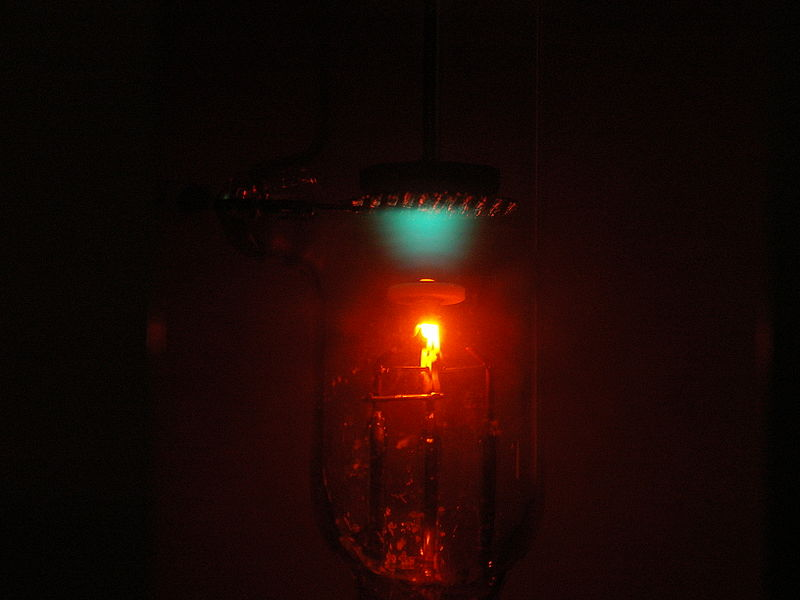
\includegraphics[width=7cm]{bilder/fhz0}}
\label{wtd}
\end{minipage}
\end{center}

\vspace{7cm}
\noindent
\begin{center}
\begin{tabular}{r l}
Tutor & Heimberger\\
Durchführung & 29. Mai 2013 von 14-18 Uhr \\

E-Mail Dominik & dominik.wille@fu-berlin.de \\
E-Mail Alexander & Matthias.Heinisch@gmx.de \\
\end{tabular}
\end{center}

\newpage
\tableofcontents
\newpage

\section{Physikalische Grundlagen}
\subsection{Atommodell}
Am Anfang des 20. Jahrhunderts entdeckten die Physiker James Frank und Gustav Hertz diskrete Anregungsstufen  von Elektronen in Quecksilber. Diese Erkenntnisse waren ein glänzender Beweis für die neue Quantenhypothese und des Bohr-Sommerfeld-Atommodells.\\
In diesem Atommodell nahm Bohr an, dass sich die Elektronen nur auf bestimmten Bahnen strahlungsfrei bewegen können. Dabei entsprechen die Bahnen einem vielfachen der DeBroglie-Wellenlänge (Materiewelle der Elektronen).\\
Demnach können ein Großteil der rechnerischen Bahnen ausgeschlossen werden und es sind nur diskrete Werte für den Drehimpuls und den Bahnradius möglich. Später fand Sommerfeld heraus, dass sich die Elektronen auch auf Ellipsenbahnen bewegen können und nicht nur, wie zuvor angenommen, auf Kreisbahnen. Damit die Bahnen eindeutig parametrisiert werden können, ordnete man ihnen die Quantenzahlen n,l,m,s zu. Dabei beschreibt die Hauptquantenzahl n die Energieniveaus der Elektronen mit den Werten n=1,2,3,... Je größer die Zahl wird, desto weiter ist der Abstand zu dem Kern des Atoms. l ist die Nebenquantenzahl, welche die Exzentrizität der Ellipse im Wertebereich \(o\leq l\leq n-1\). Die Magnetquantenzahl m beschreibt die Ausrichtung der Ellipsen, wodurch die Ellipse nun dreidimensional beschrieben ist. Die Spinquantenzahl s nimmt Werte von \(\pm\frac{1}{2}\) an und beschreibt den Eigendrehimpuls des Elektrons. Durch das Pauli-Prinzip kann nur ein Elektron jeweils ein Energieniveau besetzten.

\subsection{Termschema}
Die Elektronen befinden sich bekanntlich auf verschiedenen Energieniveaus, welche von Innen (niedrige Energie) nach Außen (hohe Energie) besetzt werden. Diese Elektronen können durch Anregung auf ein höheres Energieniveau gehoben werden. Wenn die angeregten Elektronen wieder auf ihren Grundzustand zurückfallen, emittieren sie Photonen, deren Wellenlänge der Energiedifferenz der Niveaus entspricht. Die folgende Abbildung veranschaulicht, über welche Niveaus ein Elektron auf seinen Grundzustand zurückfallen kann:

{\begin{center}
\begin{minipage}{\linewidth}
\centering
\makebox[0cm]{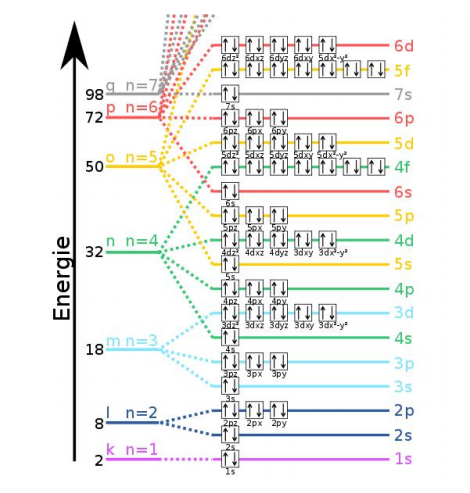
\includegraphics[width=7cm]{bilder/fhz2}}
\captionof{figure}{Allgemeines Termschema}%
\label{wtd}
\end{minipage}
\end{center}

\subsection{Frank-Hertz-Versuch}
{\begin{center}
\begin{minipage}{\linewidth}
\centering
\makebox[0cm]{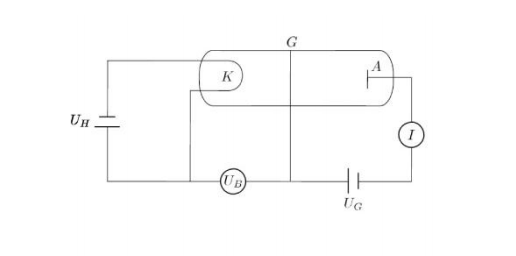
\includegraphics[width=7cm]{bilder/fhz1}}
\captionof{figure}{Versuchsaufbau}%
\label{wtd}
\end{minipage}
\end{center}
Bei diesem Experiment hatten sie eine mit Quecksilberdampf gefüllte Röhre, in welcher Elektronen von einer Glühkathode K aus beschleunigt werden und durch ein Gitter G zu einer Auffangelektrode A gelangen. Die Beschleunigung erfolg mithilfe einer Heizspannung \(U_H\). Sie ist bedeutend größer als die zwischen dem Gitter und der Anode anliegenden Bremsspannung \(U_G\)\\
Anfangs erfolgen nur elastische Stöße der Elektronen mit dem Quecksilber und im Auffängerkreis ist eine gleichmäßig zunehmender Stromfluss messbar. Erreicht die Beschleunigungsspannung jedoch einen Schwellenwert bzw. ihr ganzzahliges Vielfaches, so bricht der Strom ab und steigt anschließend wieder von neuem an.\\
Im Praktikum werden wir Bariumoxidkathoden benutzen und die in der Röhre angeordneten Elektroden sind planparallel angeordnet. Der Abstand zwischen Kathode und Anode ist größer als die mittlere freie Wellenlänge, wodurch die Stoßwahrscheinlichkeit erhöht wird.

\section{Aufgaben}
\subsection*{Aufgabe 1}
Beobachtung der Elektronenstoß-Anregungskurve (Frank-Hertz-Kurve) von Quecksilber bei einer (Ofen-)Temperatur von etwa 190\(^\circ\)C mit dem Oszilloskop. Optimierung der Kurve durch geeignete Einstellungen der experimentellen Parameter (Ofenheizung, Kathodenheizung, Beschleunigungsspannung)

\subsection*{Aufgabe 2}
Quantitative Aufnahme der Kurve mit einem X-Y-Schreiber. Bestimmung der zugehörigen Übergangsenergie in Quecksilber.

\subsection*{Aufgabe 3}
Beobachtung und Registrierung weiterer Anregungskurven für Temperaturen von 150 und 210\(^\circ\)C. Qualitative Diskussion der Ergebnisse.

\subsection*{Aufgabe 4}
Aufnahme und Auswertung einer Frank-Hertz-Kurve für Neon bei Zimmertemperatur.

\newpage
\section{Aufgabe 1}
\begin{center}
\begin{minipage}{\linewidth}
\centering
\makebox[0cm]{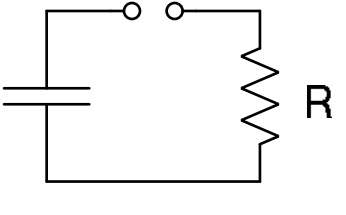
\includegraphics[scale=0.5]{sb1}}
\captionof{figure}{Schaltplan Aufgabe 1}%
\label{schaltplan_nr1}
\end{minipage}
\end{center}

Für diese Aufgabe haben wir einen Kondensator mit einem Widerstand in Reihe geschalten (siehe Abbildung 1.1). Mit einem Frequenzgenerator legten wir eine Spannung an und mit Hilfe eines Oszilloskops veränderten wir die Frequenz, bis beide Sinuskurven die gleiche Spannung hatten. 
Damit die Teilspannung an der Spule und am Kondensator übereinstimmen muss folgendes gelten:
\begin{equation}
U_C = U_R 	\Rightarrow	 U_{ges} = U_C + U_R
\end{equation}
Mit einem Spannungsmessgerät (Fluke 175) haben wir die Spannung zwischen dem Widerstand und dem Kondensator gemessen. Dabei betrug der Spannungsunterschied:
\begin{equation}
\notag
\Delta U=0,023 V
\end{equation}

Die Frequenz betrug dabei konstant:

\begin{equation}\notag
f_{char} = (160,45\pm 0,1) Hz
\end{equation}

Die verwendeten Bauteile des R-C-Kreises wurden separat noch einmal nachgemessen, dabei ergab sich für den Widerstand einen Wert von:
\begin{equation}\notag
R = (0.990 \pm 0.012)k\Omega
\end{equation}

und die Kapazität des Kondensators:
\begin{equation}\notag
C = (1.001 \pm 0.013)\mu F
\end{equation}

Die Fehler errechnen sich aus $\pm (1.0\% +3dgt)$.

\subsection{Berechnung der Frequenz}
Nun können wir über folgende Formel den theoretischen Wert der Frequenz f berechnen:
\begin{equation}\notag
f_{theo}=\frac{1}{2\pi RC}= (160.6 \pm 2.0)Hz
\end{equation}

Den Fehler bestimmen wir über die Gauß'sche Fehlerfortpflanzung:
\begin{equation}\notag
\Delta f_{theo}=\sqrt{\left(\frac{\partial f_{theo}}{\partial R}\cdot \Delta R\right)^2+\left(\frac{\partial f_{theo}}{\partial C}\cdot \Delta C\right)^2}
\end{equation}

\subsection{Phasenverschiebung}
Für die Phasenverschiebung haben wir bei einer Frequenz von f = 160,30 HZ am Oszilloskop ein \(\Delta\)t = 0,8ms abgelesen. Dafür ergibt sich für \(\phi\) einen Wert für:
\begin{equation}
\notag
\phi = 2\pi f \Delta t = (0,806 \pm 0,009)^\circ = (0,257\pm 0,003)\pi
\end{equation}

Somit ergibt sich wie erwartet \(\frac{\pi}{4}\) für die Phasenverschiebung.
Um nun noch die Phasenverschiebung auszurechnen, benutzten wir:
\begin{equation}\notag
\phi_{theo}=arctan\left(\frac{1}{\omega RC}\right)=\left(0,7854 \pm 0.0065\right)^\circ =(0,250\pm 0,003)\pi
\end{equation}

Den Fehler bekommen wir aus:
\begin{equation}\notag
\Delta \phi_{theo}=\sqrt{\left(\frac{\partial \phi_{theo}}{\partial f_{theo}}\cdot \Delta f_{theo}\right)^2+\left(\frac{\partial \phi_{theo}}{\partial C}\cdot \Delta C\right)^2+\left(\frac{\partial \phi_{theo}}{\partial R}\cdot \Delta R\right)^2}
\end{equation}

\subsection*{Fazit}
Den Wert für die charakteristische Frequenz konnten wir relativ schnell finden, nachdem wir festgestellt hatten, dass ein Messgerät einen Wackelkontakt hatte und bis dahin nur seltsame Werte geliefert wurden.\\
Der theoretische und der gemessene Wert der charakteristische Frequenz sind gleich, nur dass der Fehler des theoretischen Werts aufgrund der Bauteile doch relativ groß ist. Die Phasenverschiebung ist auch ziemlich klein.
\section{Aufgabe 2}
\subsection{Abschätzung des Arbeitswiderstandes}

Um den Arbeitswiderstand zu bestimmen, benutzen wir das Vier-Quadranten-Kennlinienfeld (Abbildung 7) und gehen vom äußersten Punkt des dritten Quadranten für \(I_B\)= 140,8\(\mu A\) senkrecht nach oben. Im Zweiten Quadranten treffen wir so den Wert für \(I_C\)=13,9 mA, welches unser Startpunkt der Arbeitsgeraden (bzw. Kollektor-Widerstandsgerade) sein wird. Damit ergeben sich die Koordinaten (\(U_{CE}\) = 0[V], \(I_{C}\) = 13,9[mA]) für den Punkt \(P_1\) des Kurzschlussfalls. Der Punkt \(P_2\) liegt bei den Koordinaten (\(I_{C}\) = 0 [mA],\(U_{CE}\) = 12[V]), weil 12[V] die maximale Versorgungsspannung betrug.\\
Der Arbeitspunkt \(P_{A}\) liegt laut Definition bei \(\left(\frac{U_{CE}}{2}, \frac{I_{C}}{2}\right)\), welches bei uns den Werten (6.055[V],6.95[mA]) entspricht.\\

Den Arbeitswiderstand wird über die Formel:
\begin{equation}
\notag
R_{A}=\mid \frac{1}{m}\mid = \left(\frac{U_{EC}}{I_C}\right) = 871.23 \Omega
\end{equation}\\

Während des Versuchs haben wir für den Arbeitswiderstand einen Wert von (\(464.3\pm 2.6)\Omega\) gemessen.\\

Der Basisvorwiderstand ergibt sich aus der Formel:
\begin{equation}
\notag
R_V= \frac{U_{EC}-U_{EB}}{I_B}=\frac{6V-0.7V}{(63.5\cdot 10^{-6})A}=83.5k\Omega
\end{equation}

Hier hatten wir einen Wert von (\(100.2\pm 0.8)k\Omega\) gemessen. Auf die Unterschiede dieser Werte werden wir später in der Diskussion eingehen.

\subsection{Überprüfung der Kollektor-Widerstandsgeraden}

Nun überprüfen wir die abgeschätzten Werte, indem wir einen Arbeitswiderstand und einen Basisvorwiderstand in die Schaltung einbauen (siehe Abbildung 6) und eine neue Messreihe aufnehmen. Wir steigern dabei die Werte für \(I_B\) in gleichen Abständen und notieren, wie sich die anderen Größen dazu verhalten. \(U_0\) hielten wir konstant auf (\(12.11\pm 0.09\))

\newpage
Unsere Messung ergaben folgende Werte:\\

\begin{center}
\begin{tabular}{r r r r}
\(I_B [\mu A]\) & \(I_C [mA]\) & \(U_B [V]\) & \(U_{CE}[V]\) \\
\hline
\(52.116\) & \(9.0\) & \(0.116\) & \(7.93\) \\ 
\(62.519\) & \(9.3\) & \(0.191\) & \(7.75\) \\ 
\(72.518\) & \(9.7\) & \(0.255\) & \(7.59\) \\ 
\(81.305\) & \(10.0\) & \(0.315\) & \(7.45\) \\ 
\(94.132\) & \(10.5\) & \(0.362\) & \(7.22\) \\ 
\(101.505\) & \(10.9\) & \(0.429\) & \(7.01\) \\ 
\(113.423\) & \(11.8\) & \(0.526\) & \(6.61\) \\ 
\(122.311\) & \(12.6\) & \(0.586\) & \(6.24\) \\ 
\(131.906\) & \(22.7\) & \(0.755\) & \(1.52\) \\ 
\(142.410\) & \(23.4\) & \(0.757\) & \(1.17\)
\end{tabular}
\captionof{table}{Rohmesswerte für Aufgabe 2.2}
\end{center}

\section{Aufgabe 3}
In dieser Aufgabe wurde eine Wechselstrombrücke aufgebaut um sowohl die Induktivität \(L_x\) als auch den Ohmschen Widerstand \(R_x\) der Spule vom Tiefpass aus Aufgabe 2 zu bestimmen. 

\subsection{Aufbau}
Hierfür wurde eine Schaltung auf dem Steckbrett nach folgendem Schaltplan aufgebaut. Die Phase zwischen den beiden Spannungsmesspunkten wurde mit dem Oszilloskop mit der ,,elliptischen Auftragung'' auf \(\varphi = 0 \) eigestellt. Und anschließend die Effektivspannung mit dem Fluke 175 gemessen
\begin{center}
\begin{minipage}{\linewidth}
\centering
\makebox[0cm]{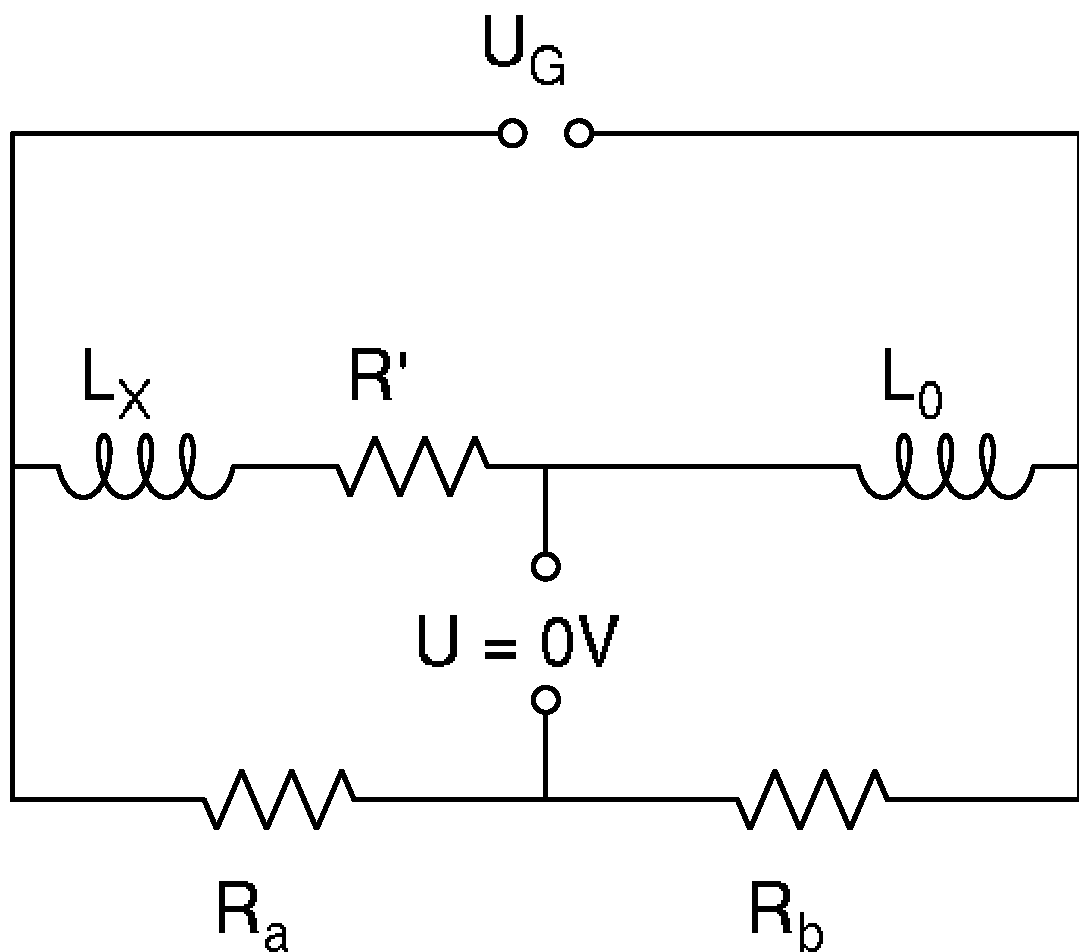
\includegraphics[width=6cm]{bruecke}}
\captionof{figure}{Schaltplan der Wechselstrombrücke}
\end{minipage}
\end{center}

\subsection{Gegebenes und Messwerte}
Separat wurden folgende Größen gemessen oder von den Aufschriften der Bauteile entnommen. Leider wurde vergessen zu notieren mit welchem Messgerät die Widerstände gemessen wurden die Fehler werden mit \(\Delta R = 1\% + 5d\) abgeschätzt.
\begin{center}
\begin{tabular}{c|c}
Messgröße & Messwert\\\hline
\(f\) & \((1999 \pm 14)\, Hz \) \\
\(L_0\) & \((1,507 \pm 0,020)\, mH \) \\
\(R_0\) & \((2,91 \pm 0,02)\, \Omega \) \\
\(R_a\) & \((761 \pm 13)\, \Omega \) \\
\(R_b\) & \((241,8 \pm 2,9)\, \Omega \) \\
\(R'\) & \((5,3 \pm 0,5)\, \Omega \) \\
\(f\) & \((1999 \pm 14)\, Hz \) \\ \hline
\(R_x\) & \(\left(3,7 \pm 0,5 \right)\, \Omega \) \\
\(L_x\) & \((4,82\pm 0,07)\, mH \) \\
\end{tabular}
\captionof{table}{Sepperate Messung aller Größen}%
\end{center}

\subsection{Auswertung}
Um nun aus den Vorhanden Messdaten \(L_x\) und \(R_x\) zu bestimmen, wird folgender Ansatz gemacht:
\begin{align}
\frac{Z_a}{Z_b} &= \frac{i\omega L_x + R'+ R_x}{i\omega L_0 + R_0}
\end{align}
Da über den Phasenabgleichswiderstand die Phase auf \(\varphi = 0\) gebracht wurde müssen die beiden Phasenverschiebungen der Spulen und Widerständen identisch sein. Daher gilt:
\begin{align}
\Rightarrow \frac{i\omega L_0}{R_0} &= \frac{i\omega L_x}{R'+R_x}\notag \\
\Rightarrow L_x &= \frac{L_0}{R_0}\cdot\left( R' + R_x \right) \label{L_x}
\end{align}
Außerdem wurden \(R_a\) und \(R_b\) derart gewählt, dass gelten muss:
\begin{align}
\frac{R_a}{R_b} &= \frac{\omega L_x + R' + R_x}{\omega L_0 + R_0}
\end{align}
Nach einsetzten von \eqref{L_x} formt sich das zu
\begin{equation}
R_x = \frac{R_a}{R_b} \cdot R_0 - R'
\end{equation} um.
Für die Fehler gilt nach Gaußscher Fehlerfortpflanzung:
\begin{align}
\Delta R_x &= \sqrt{
\left( \frac{R_0}{R_b} \cdot \Delta R_a \right)^2 +
\left( \frac{R_a}{R_b} \cdot \Delta R_0 \right)^2 +
\left( \frac{R_a}{R_b^2} \cdot \Delta R_b \right)^2 +
\left( \Delta R' \right)^2
}\notag \\
\Delta L_x &= \sqrt{
\left( \frac{R'+R_x}{R_0} \Delta L_0 \right)^2 +
\left( \frac{L_0\left( R'+R_x \right)}{R_0^2}  \cdot \Delta R_0 \right)^2 +
\left( \frac{L_0}{R_0} \cdot \Delta R' \right)^2 +
\left( \frac{L_0}{R_0} \cdot \Delta R_x \right)^2
}\notag
\end{align}
Ausgerechnet ergibt das:
\begin{center}
\begin{tabular}{c|c}
Messgröße & Errechneter Wert\\\hline
\(R_x\) & \(\left(3,86 \pm 0,23 \right)\, \Omega \) \\
\(L_x\) & \((4,74\pm 0,50)\, mH \) \\
\end{tabular}
\captionof{table}{Mit der Apparatur ermittelte Größen}
\end{center}

\subsection{Fazit}
Die ermittelten werte für die Induktivität und den ohmschen Widerstand der Spule sind identisch zu den direkt mit dem Messgerät gemessenen Werten. dabei konnte sogar die Genauigkeit der Widerstandsmessung der Spule erhöht werden, da diese sonst nur mit dem für kleine Widerstände sehr ungenauem VC230 oder Fluke 175 gemessen werden konnten.
\begin{center}
\begin{tabular}{c|c|c}
Messgröße & Errechneter Wert & Vergleichswert\\\hline
\(R_x\) & \(\left(3,9 \pm 0,3 \right)\, \Omega \) &  \(\left(3,7 \pm 0,5 \right)\, \Omega \)\\
\(L_x\) & \((4,7\pm 1,7)\, mH \) & \((4,82\pm 0,07)\, mH\) \\
\end{tabular}
\captionof{table}{Mit der Apparatur ermittelte Größen}
\end{center}

\section{Fazit}
Alle drei Aufgaben waren sehr gut durchführbar. Alle Geräte haben durchgehend funktioniert und waren leicht zu bedienen. Besonders das moderne Oszilloskop sorgte für vergleichsweise gute Messdaten. Die Ergebnisse waren zufriedenstellend und wir können die Versuche zu den Wechselstromkreisen auf jeden Fall zu den angenehmen und gleichzeitig interessanten Versuchen zählen.
\section{Aufgabe 4}
Das Vorgehen in Aufgabe 4 ist völlig identisch zu dem in Aufgabe 1-3, mit dem Unterschied, dass eine Neonröhre verwendet wird statt einer Quecksilberröhre. Der Aufbau, Durchführung und Fehlerrechnung können aus den vorherigen Aufgaben übernommen werden.
\subsection{Graphen/Messwerte}
Die Messwerte wurden wieder exportiert und mit GNU-Plot aufgetragen, die Minimalstellen wurden mit dem Auge geschätzt.
\begin{center}
\begin{minipage}{\linewidth}
\centering
\makebox[0cm]{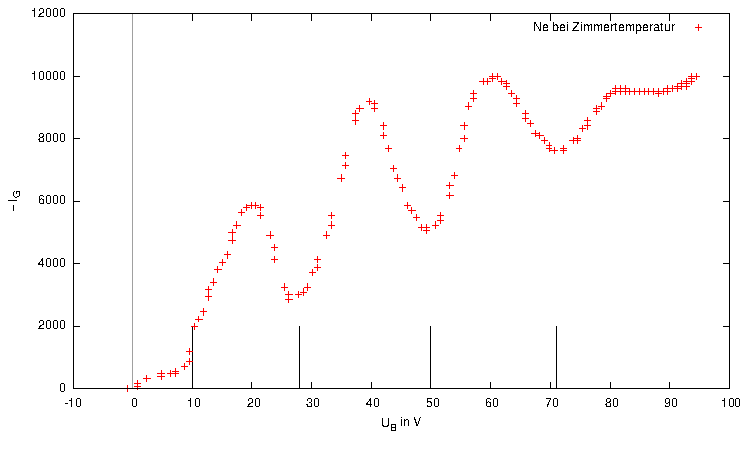
\includegraphics[width=\textwidth]{graphen/a3/a3}}
\captionof{figure}{Franck-Hertz-Kurve von Neon}
\label{a3}
\end{minipage}
\end{center}
Die so gefunden Spannungen \(U_B\) der Minima werden nun tabelliert und anschließend mit einer linearen regression dargestellt um die Steigung \(b\) des als linear angenommen Verlaufs zu erhalten.
\begin{center}
\begin{tabular}{c|c}
Minimum & \(U_B\)\\\hline
\(0\) & \(10\, V\)\\
\(1\) & \(28\, V\)\\
\(2\) & \(50\, V\)\\
\(3\) & \(71\, V\)\\
\end{tabular}
\captionof{table}{Minima von \(U_B\) der aufgenommenen Franck-Hertz-Kurven von Neon}
\end{center}
\begin{center}
\begin{minipage}{\linewidth}
\centering
\makebox[0cm]{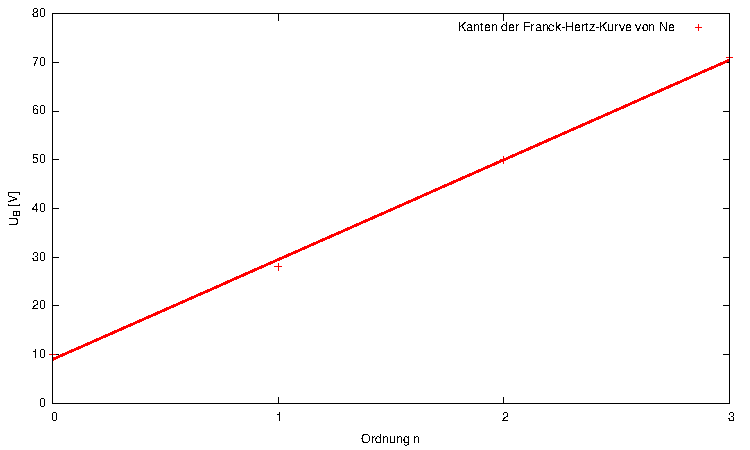
\includegraphics[width=\textwidth]{graphen/a3/graph}}
\captionof{figure}{Minima der Franck-Hertz-Kurve von Neon}
\label{graph_a3}
\end{minipage}
\end{center}
Die Steigung wurde ermittelt zu:
\begin{align}
b = \left( 20,50 \pm 0,59 \right)\, V \notag
\end{align}
\subsection{Auswertung}
Auch die Auswertung läuft wieder völlig analog zu den Aufgaben 1-3.
Die Steigung \(b\) kann also wieder wie in \eqref{E_kin} direkt in eine Energie übersetzt werden, daher gilt für die Anregungsenergie von Neon:
\begin{align}
E = \left( 20,50 \pm 0,59 \right)\, eV \notag
\end{align}
\subsection{Zwischenfazit}
Neon ist bei Zimmertemperatur gasförmig und es wird daher keine weitere Heizung benötigt um den Abstand der Atome hinreichend zu vergrößern. Die ermittelte Anregungsenergie von \(\left( 20,5 \pm 0,6\right)\, eV \) ist identisch zum Literaturwert von \(\left( 18,7 \pm 0,3\right)\, eV \), da die Fehlerintervalle überlappen. Bei Neon geht der Zustand über diverse Nebenzustände zurück in den Grundzustand, weswegen auch ein größeres Intervall für die Anregungsenergie angegeben wird. Beim zurückgehen in den Grundzustand wird auch unter andrem das sichtbare rote Licht emittiert.

\section{Fazit}

\end{document}
